% 第3章第1节：最短路（路径成本与三类距离结果、距离标签与松弛、DAG递推、Bellman--Ford、Dijkstra、方法比较与结果检验）。

\section{最短路}
\label{sec:graph-shortest-paths}

第~\ref{sec:graph-bfs}节的广度优先遍历给出从起点出发的最少边数。可是在道路网络中，每段路的长度不同；在任务调度中，从一个状态转到另一个状态的代价也各不相同。这时要比较的是路线上各段数值之和，经过的边数少不等于总成本低。

本节在有向加权图上研究这个问题。先说明路线成本怎样定义、距离可能出现哪几类结果，再建立三种算法共用的距离标签与松弛操作。随后依次介绍三种算法：有向无环图上的递推利用无环次序，Bellman--Ford算法允许标签反复修正，Dijkstra算法在边长非负时永久确定标签。每种算法的正确性论证紧接在各自的机制之后，最后比较三者的适用范围，并说明怎样检验一份最短路结果。

\subsection{路径成本与最短路问题}
\label{sec:graph-opt-path-cost}

设$\mathcal G=(V,E)$是有限有向图，每条弧$u\to v$带有一个实数\emph{长度}$\ell_{u,v}$。长度可以表示距离、时间或转换代价，也允许为负，例如某次转换带来收益。对一条行走$W=(v_0,v_1,\ldots,v_k)$，规定它的成本为沿途弧长之和：
\[
  \ell(W)=\sum_{r=1}^{k}\ell_{v_{r-1},v_r}.
\]
只含一个顶点的零步行走成本为零。所有长度都等于$1$时，成本就是边数，回到广度优先遍历的情形；一般长度下两者不再一致。例如$s$到$t$有一条长$5$的直达弧，又有经过$u$、两段各长$1$的路线，两步路线反而更短。

\paragraph{两种候选集合}
寻找“最短路线”时，必须先说清候选集合是什么。一种选择只允许简单路径，即不重复经过顶点的路径；另一种允许一般的行走，顶点和弧都可以重复。有限图中简单路径只有有限条，因此只要终点可达，最小值一定存在；行走可以无限地绕圈，候选有无穷多个，只能谈成本的下确界。

\begin{definition}[最短路问题]
\label{def:graph-opt-shortest-path}
给定有限有向图$\mathcal G=(V,E)$、弧长$\ell_{u,v}\in\mathbb R$与源点$s\in V$。对每个顶点$v$，记$\mathcal W_{s,v}$为从$s$到$v$的全部有限行走组成的集合，称
\[
  \delta(v)=\inf_{W\in\mathcal W_{s,v}}\ell(W)
\]
为$s$到$v$的\term{最短路}距离，约定空集的下确界为$+\infty$。若某条行走$W\in\mathcal W_{s,v}$满足$\ell(W)=\delta(v)$，就称$W$是一条$s$到$v$的最短路。求出全部$\delta(v)$及相应路线的问题称为单源最短路问题。
\end{definition}

本节的算法计算的都是行走下确界$\delta(v)$。在多数情形中它与简单路径的最小值一致，原因是行走中的绕圈部分可以删掉。设行走$W$两次经过顶点$x$，两次之间的一段是从$x$回到$x$的闭行走$C$，删去$C$得到更短的行走$W'$，并且$\ell(W')=\ell(W)-\ell(C)$。只要$C$的成本非负，删去它就不会增加成本。反复删除，直到不再有重复顶点，便得到一条成本不超过$\ell(W)$的简单路径。

\paragraph{负环与三类结果}
删除闭合段的论证只在闭行走成本非负时有效。成本为负的有向环称为\term{负环}（negative cycle）。若能从$s$走到某个负环，绕若干圈后再走到$v$，则每多绕一圈，成本就再降低一次，于是$\delta(v)=-\infty$。这并不表示存在一条“长度为负无穷的路径”，而是说任何有限成本都能被另一条行走打破。反过来，若没有这样“从$s$可达、又能到达$v$”的负环，那么$s$到$v$的行走中出现的任一闭合段也不可能为负。原因是一条成本为负的闭行走，在第一个重复顶点处切开，总能分出一个简单环，剩下的部分仍是闭行走；重复这一切分，闭行走的成本就写成若干个简单环的成本之和，其中必有一个为负，而这个环同样从$s$可达、又能到达$v$。因此在这种情形下，所有闭合段都可以删除，$\delta(v)$等于简单路径的最小成本，并且由一条简单路径达到。

综上，一次单源查询中，每个顶点的距离属于三类之一：不可达时$\delta(v)=+\infty$；可达且不受负环影响时$\delta(v)$为有限值，并由一条简单路径达到；能从某个$s$可达的负环到达时$\delta(v)=-\infty$。三类顶点可以出现在同一张图中。图~\ref{fig:graph-opt-distance-outcomes}中，负环$a\to b\to a$只影响它自己及其后继$t$；旁支$u$不能从这个负环到达，距离仍是有限的$4$；另一个负环$x\to y\to x$从$s$出发到不了，对本次查询没有任何影响。所以不能因为图中某处有负环，就把全部顶点都标成负无穷。

\begin{figure}[!htb]
  \centering
  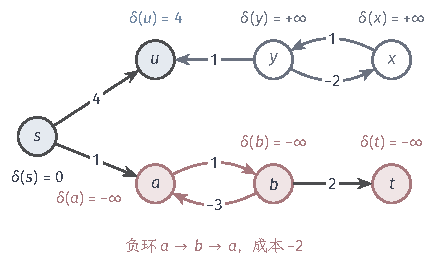
\includegraphics[width=73.801mm]{figures/01-basic-mathematics/04-graphs/tikz/c3-distance-outcomes/figure.pdf}
  \caption{单源最短路的三类结果同处一图（源点为$s$，弧旁数字为长度）。$a\to b\to a$的成本为$1-3=-2$，是从$s$可达的负环，环上的$a,b$及其后继$t$的距离为$-\infty$（红色）；旁支$u$不能从该负环到达，距离为有限值$4$（蓝色）；负环$x\to y\to x$从$s$不可达，$x,y$的距离为$+\infty$（灰色），弧$y\to u$也不会改变$u$的距离。}
  \label{fig:graph-opt-distance-outcomes}
\end{figure}

无向图中的负边需要特别注意。把无向边$\{u,v\}$换成两条同长的反向弧$u\to v$与$v\to u$以后，一条长为负的无向边自己就构成负环：沿它走过去再走回来，成本是两倍的负长度。因此，含负边的无向图不能直接套用本节的有向算法；本节默认讨论有向图，无向边只在长度非负时换成一对反向弧。

\subsection{距离标签与松弛}
\label{sec:graph-opt-relaxation}

三种算法都不直接枚举行走，而是为每个顶点保存一个当前已知的最好成本，在发现更好的路线时更新它。设想已经知道一条从$s$到$u$、成本为$d(u)$的路线，又有弧$u\to v$，那么把这条弧接在路线末尾，就得到一条到$v$、成本为$d(u)+\ell_{u,v}$的路线。如果它比$v$目前记录的成本更低，就应该改用它。

\paragraph{标签与松弛操作}
为每个顶点$v$保存一个\term{距离标签}（distance label）$d(v)\in\mathbb R\cup\{+\infty\}$和一个前驱$p(v)$。初始时令$d(s)=0$，其余顶点$d(v)=+\infty$，前驱为空。对一条弧$u\to v$执行\term{松弛}（relaxation），是指比较当前标签$d(v)$与候选值$d(u)+\ell_{u,v}$：若$d(u)<+\infty$且
\[
  d(u)+\ell_{u,v}<d(v),
\]
就令$d(v)\leftarrow d(u)+\ell_{u,v}$、$p(v)\leftarrow u$；否则什么也不做。只有严格改善时才更新，因而标签只会下降，不会上升。

松弛只从有限标签出发延长路线，由此得到所有算法共用的一个不变量：\emph{每个有限标签$d(v)$都等于某条从$s$到$v$的行走的成本}。初始时只有$d(s)=0$有限，对应零步行走。若松弛把$d(v)$改为$d(u)+\ell_{u,v}$，则把$u$的那条行走接上弧$u\to v$，就得到成本恰为新标签的行走。由此立即得到$d(v)\geq\delta(v)$：标签永远是真实距离的上界。后面每种算法要做的，都是说明在适当的条件下，这个上界最终会降到$\delta(v)$。

图~\ref{fig:graph-opt-relaxation}画出一次松弛。左图中$v$原来经由$w$得到标签$8$；检查弧$u\to v$时，候选值$3+2=5$更小，于是标签改为$5$，前驱同时改为$u$。右图中$v$的标签已是$4$，候选值$5$不能改善它，标签和前驱都保持不变。距离数组和前驱数组必须同步修改：如果只改距离而不改前驱，回溯得到的路线成本就不再等于标签。

\begin{figure}[!htb]
  \centering
  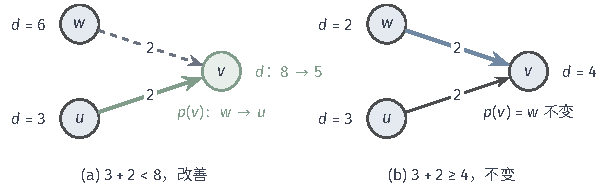
\includegraphics[width=102.993mm]{figures/01-basic-mathematics/04-graphs/tikz/c3-relaxation/figure.pdf}
  \caption{对弧$u\to v$松弛（顶点旁为当前标签，弧旁为长度）。(a) 候选值$d(u)+\ell_{u,v}=3+2=5$小于原标签$8$，标签改为$5$，前驱由$w$改为$u$（绿色表示被改善的标签与新的前驱弧，虚线为被替换的旧前驱弧）。(b) 原标签为$4$，候选值$5$不能改善，标签与前驱都不变。}
  \label{fig:graph-opt-relaxation}
\end{figure}

\paragraph{局部等式不能单独确定距离}
若没有可达负环，真实距离满足一组局部等式：$\delta(s)=0$，并且对每个可达的$v\neq s$，有$\delta(v)=\min_{u\to v}\{\delta(u)+\ell_{u,v}\}$。这只是说最短路的最后一条弧总来自某个前驱。但满足这组等式的数组不一定就是距离。设$s\to a$长$5$，$a\to b$与$b\to a$长都为$0$，则对任意$c\leq5$，取$D(s)=0$、$D(a)=D(b)=c$都满足
\[
  D(a)=\min\{D(s)+5,\ D(b)+0\}=c,\qquad D(b)=D(a)+0=c,
\]
而真实距离是$\delta(a)=\delta(b)=5$。这里的零成本环让$a,b$互相“支撑”着一个过低的值，却没有任何实际路线达到它。所以算法不能只去求解局部等式，而要从“源为零、其余为无穷”的初值出发，只沿实际路线下调标签，上面的不变量保证了这一点。初值保证标签不会无中生有，松弛保证每个标签都有路线见证，而松弛按什么次序进行、何时可以停止，则由各算法分别规定。

\paragraph{距离、前驱与访问状态}
算法通常维护三类数组，它们承担不同的职责。距离数组记录当前上界；前驱数组记录达到这个上界的最后一条弧，用于事后恢复路线；访问状态则记录算法自身的进度，例如Dijkstra算法中哪些顶点已经永久确定。前驱数组只在标签不再变化以后才能放心回溯。在一般有环图中，计算中途的前驱指针可能尚未形成从$s$出发的树；若存在可达负环，前驱指针甚至可能首尾相接成环。对于后面按轮次定义的递推，前驱还应与相应的轮次一同保存，才能把它们当作可回溯的路线。

\subsection{有向无环图上的最短路}
\label{sec:graph-opt-dag-shortest-path}

在一般的图中，一个顶点的标签可能在它的出弧已被松弛之后才下降，这时它的后继也必须随之更新。有向无环图没有这个问题：第~\ref{sec:graph-topological-order}节说明，有限有向无环图存在拓扑序，使每条弧的起点排在终点之前。按拓扑序处理顶点，轮到$v$时，所有指向$v$的弧都已被松弛，$v$的标签此后不会再变。

\begin{algorithm}[有向无环图上的最短路]
\label{alg:graph-opt-dag-shortest-path}
输入：有限有向无环图、弧长$\ell_{u,v}\in\mathbb R$、源点$s$。输出：全部距离$\delta(v)$与前驱$p(v)$。
\begin{enumerate}
  \item 求一个拓扑序$v_1,\ldots,v_n$；令$d(s)=0$，其余$d(v)=+\infty$，前驱为空。
  \item 按$i=1,\ldots,n$的顺序处理$v_i$：若$d(v_i)<+\infty$，对其每条出弧$v_i\to w$执行松弛。
  \item 对标签有限的顶点，沿前驱从终点退回$s$再反转，得到一条最短路；标签为$+\infty$的顶点报告不可达。
\end{enumerate}
\end{algorithm}

\paragraph{算例}
取弧$s\to a$长$2$、$s\to b$长$5$、$a\to b$长$-1$、$a\to t$长$5$、$b\to t$长$2$，它没有有向环，拓扑序可取$(s,a,b,t)$。处理$s$时，$a$的标签由$+\infty$改为$2$，$b$的标签由$+\infty$改为$5$。处理$a$时，候选$2+(-1)=1<5$使$b$改为$1$，同时$t$由$+\infty$改为$2+5=7$。处理$b$时，候选$1+2=3<7$使$t$改为$3$。最后处理$t$，它没有出弧。前驱为$p(a)=s$、$p(b)=a$、$p(t)=b$，从$t$回溯得到最短路$s\to a\to b\to t$，成本$2-1+2=3$。图~\ref{fig:graph-opt-dag-labels}记录了这个过程中各标签的变化。

\begin{figure}[!htb]
  \centering
  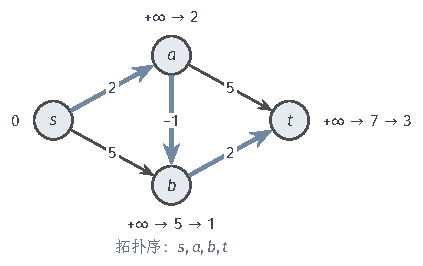
\includegraphics[width=71.635mm]{figures/01-basic-mathematics/04-graphs/tikz/c3-dag-labels/figure.pdf}
  \caption{按拓扑序$(s,a,b,t)$在有向无环图上松弛。顶点旁列出标签的变化次序，例如$b$先由处理$s$得到$5$，再由处理$a$改为$1$；蓝色粗弧是最终前驱弧，组成最短路$s\to a\to b\to t$（成本$3$）。负长度弧$a\to b$并不妨碍计算，因为正确性只依赖无环次序。}
  \label{fig:graph-opt-dag-labels}
\end{figure}

\paragraph{正确性}
上面的过程之所以能一遍完成，是因为处理到某个顶点时，所有可能到达它的路线都已考虑过。下面把这一点写成归纳证明。

\begin{theorem}[有向无环图上最短路的正确性]
\label{thm:graph-opt-dag-shortest-path}
设$\mathcal G$是有限有向无环图，弧长为任意实数。算法~\ref{alg:graph-opt-dag-shortest-path}结束时，对每个顶点$v$都有$d(v)=\delta(v)$；其中$\delta(v)=+\infty$当且仅当$v$从$s$不可达，其余$\delta(v)$均为有限值。
\end{theorem}

\begin{proof}
有向无环图中的行走不会重复顶点，因此每条行走都是简单路径，只有有限条，$\delta(v)$只可能是$+\infty$或有限值。松弛只改变弧终点的标签，而指向$v$的弧都从拓扑序中排在$v$之前的顶点出发，所以轮到$v$时它的标签已经不再改变。下面对拓扑序归纳，证明轮到$v$时$d(v)=\delta(v)$。

排在$s$之前的顶点从$s$不可达，它们的标签保持$+\infty$，与距离一致。对$v=s$，不存在回到$s$的非零步行走，故$\delta(s)=0=d(s)$。设$v$排在$s$之后，并且此前的顶点都已满足结论。若$v$不可达，则它的标签不可能变为有限值，因为有限标签总对应一条实际行走。若$v$可达，任取一条$s$到$v$的路径，设其最后一条弧为$u\to v$，则$u$排在$v$之前，路径前缀的成本不小于$\delta(u)$，归纳假设给出$\delta(u)=d(u)$。处理$u$时弧$u\to v$已被松弛，因而
\[
  d(v)\leq d(u)+\ell_{u,v}=\delta(u)+\ell_{u,v}\leq\text{该路径的成本}.
\]
路径是任取的，所以$d(v)\leq\delta(v)$。结合标签不变量$d(v)\geq\delta(v)$，得$d(v)=\delta(v)$。
\end{proof}

证明中只用到“前驱先于后继处理”，没有用到边长的符号，所以负长度弧不会造成任何问题。求拓扑序需要$O(n+a)$时间，之后每个顶点处理一次、每条弧松弛一次，总时间为$O(n+a)$，标签、前驱与拓扑序共占$O(n)$额外空间。

\paragraph{扩展示例：编辑距离}
许多递推问题的状态之间天然形成有向无环图，这时就是本小节的最短路问题。比较两段序列时，常问把序列$\bm a=(a_1,\ldots,a_p)$改写成$\bm b=(b_1,\ldots,b_q)$最少需要多少次单元素操作，允许的操作是插入一个元素、删除一个元素和把一个元素替换为另一个。以$(i,j)$表示“已把$\bm a$的前$i$个元素改写成$\bm b$的前$j$个元素”这一状态，最后一步只有三种可能：删去$a_i$，从$(i-1,j)$而来，成本为$1$；插入$b_j$，从$(i,j-1)$而来，成本为$1$；让$a_i$对应$b_j$，从$(i-1,j-1)$而来，相同时成本为$0$，不同时为一次替换，成本为$1$。于是最少操作数$E(i,j)$满足
\begin{equation}
  E(i,j)=\min\bigl\{E(i-1,j)+1,\ E(i,j-1)+1,\ E(i-1,j-1)+\mathbb I\{a_i\neq b_j\}\bigr\},
  \label{eq:graph-opt-edit-distance}
\end{equation}
边界为$E(i,0)=i$、$E(0,j)=j$，其中$\mathbb I\{\cdot\}$在条件成立时取$1$、否则取$0$。

每条状态弧都使$i+j$增加，所以状态图没有有向环，$E(p,q)$就是从$(0,0)$到$(p,q)$的最短路距离，称为两段序列的\term{编辑距离}（edit distance）。按$i+j$递增或逐行的顺序计算，正是在按拓扑序松弛。例如$\bm a=(A,B)$、$\bm b=(A,C,B)$时，三行表值依次为$(0,1,2,3)$、$(1,0,1,2)$、$(2,1,1,1)$，沿“匹配$A$、插入$C$、匹配$B$”得到距离$1$。全表连同前驱需要$O(pq)$时间与空间；只要距离值时保留相邻两行即可。更一般的序列对齐与动态时间规整留到信号与序列的应用部分，这里只说明它们的计算骨架是有向无环图上的最短路。

\subsection{Bellman--Ford算法}
\label{sec:graph-opt-bellman-ford}

图中有环时没有拓扑序可用：一个顶点的标签可能在它的出弧已被松弛之后才下降，一遍扫描不够。最直接的补救是反复扫描全部弧，直到标签不再变化。为了说清楚每一轮扫描得到了什么，先讲各轮彼此分开的同步版本。

\paragraph{同步递推}
令$d^{(0)}(s)=0$，其余$d^{(0)}(v)=+\infty$。第$k$轮只读取上一轮的标签，对每个顶点比较“沿用旧值”与“在上一轮的某条路线后再接一条弧”：
\begin{equation}
  d^{(k)}(v)=\min\Bigl\{d^{(k-1)}(v),\ \min_{u\to v}\bigl(d^{(k-1)}(u)+\ell_{u,v}\bigr)\Bigr\},\qquad k=1,2,\ldots,
  \label{eq:graph-opt-bellman-ford}
\end{equation}
没有入弧时内层最小值取$+\infty$。实现上，每轮先复制上一轮的标签数组，再逐弧用旧数组计算候选值、更新新数组。这样定义的标签有一个清楚的含义。

\begin{lemma}[同步标签的含义]
\label{lem:graph-opt-bellman-ford-k-arcs}
对每个$k\geq0$与每个顶点$v$，$d^{(k)}(v)$等于从$s$到$v$、至多含$k$条弧的全部行走的最小成本；没有这样的行走时为$+\infty$。
\end{lemma}

\begin{proof}
对$k$归纳。$k=0$时，至多零条弧的行走只有$s$处的零步行走，与$d^{(0)}$一致。设结论对$k-1$成立。一条至多含$k$条弧、到达$v$的行走，要么至多含$k-1$条弧，其成本不小于$d^{(k-1)}(v)$；要么恰含$k$条弧，去掉最后一条弧$u\to v$后剩下至多$k-1$条弧、到达$u$的前缀，其成本不小于$d^{(k-1)}(u)+\ell_{u,v}$。所以全部候选的最小值不小于式~\eqref{eq:graph-opt-bellman-ford}的右端。反过来，右端每一项都由归纳假设对应一条至多$k$条弧的行走，最小值能够达到。故两者相等。
\end{proof}

沿用上一小节的四点图，并把它看成一般的有向图，按式~\eqref{eq:graph-opt-bellman-ford}逐轮计算，结果见表~\ref{tab:graph-opt-bellman-ford-rounds}。第$1$轮只能用一条弧，得到$a=2$、$b=5$；第$2$轮允许两条弧，$b$经$a$降到$1$，$t$经$a$得到$7$；第$3$轮$t$经$b$降到$3$；第$4$轮不再变化。每一列恰好是“至多$k$条弧”的最优值，例如$d^{(2)}(t)=7$对应两弧路线$s\to a\to t$，而三弧路线$s\to a\to b\to t$要到第$3$轮才被计入。

\begin{table}[!htb]
  \centering
  \caption{同步Bellman--Ford在四点图（$s\to a$长$2$，$s\to b$长$5$，$a\to b$长$-1$，$a\to t$长$5$，$b\to t$长$2$）上的逐轮标签。第$k$行是至多$k$条弧的最小成本，括号内为该轮改变标签时的前驱。}
  \label{tab:graph-opt-bellman-ford-rounds}
  \begin{tabular}{ccccc}
    \toprule
    轮次$k$ & $d^{(k)}(s)$ & $d^{(k)}(a)$ & $d^{(k)}(b)$ & $d^{(k)}(t)$ \\
    \midrule
    $0$ & $0$ & $+\infty$ & $+\infty$ & $+\infty$ \\
    $1$ & $0$ & $2$（$s$） & $5$（$s$） & $+\infty$ \\
    $2$ & $0$ & $2$ & $1$（$a$） & $7$（$a$） \\
    $3$ & $0$ & $2$ & $1$ & $3$（$b$） \\
    $4$ & $0$ & $2$ & $1$ & $3$ \\
    \bottomrule
  \end{tabular}
\end{table}

\paragraph{轮数上界与就地更新}
需要多少轮？对不受可达负环影响的顶点$v$，第~\ref{sec:graph-opt-path-cost}节说明$\delta(v)$由一条简单路径达到，而简单路径至多经过$n$个顶点、含$n-1$条弧。由引理~\ref{lem:graph-opt-bellman-ford-k-arcs}，第$n-1$轮已经计入这条路径，所以$d^{(n-1)}(v)=\delta(v)$。若某一整轮没有任何标签改变，则此后各轮的输入都相同，标签不会再变，可以提前停止；四点图在第$4$轮发现无改善，实际只需$3$轮。

常见的实现不复制数组，而是在同一个数组上逐弧松弛，一轮中刚改善的标签可以立即被同一轮后面的弧使用，称为就地更新。按$s\to a$、$s\to b$、$a\to b$、$a\to t$、$b\to t$的顺序扫描四点图，第一轮就得到全部最终标签$(0,2,1,3)$。就地更新得到的标签仍是真实行走的成本，又对每轮都不高于同步版本的标签（对轮数归纳即可），所以$n-1$轮的上界照样成立。但“第$k$轮标签恰为至多$k$条弧的最优值”这一解释只属于同步版本，不能原样套在就地更新上：同一轮内的改善可能已经串起了多条弧。

\paragraph{负环影响的检测与传播}
完成$n-1$轮以后，不受负环影响的顶点已经得到正确距离，剩下的问题是找出哪些顶点的距离为$-\infty$。固定此时的标签$d=d^{(n-1)}$，检查所有满足$d(u)<+\infty$且$d(u)+\ell_{u,v}<d(v)$的弧$u\to v$，即再做一轮仍能改善的弧，把它们的终点称为种子。然后从全部种子出发，沿出弧做一次遍历，把遍历到的顶点都标记为$-\infty$。

\begin{theorem}[Bellman--Ford算法对三类结果的判定]
\label{thm:graph-opt-bellman-ford-negative-cycles}
在同步递推的$n-1$轮之后按上述方法标记，被标记的顶点恰好是$\delta(v)=-\infty$的顶点；其余顶点中，$d^{(n-1)}(v)=+\infty$的不可达，$d^{(n-1)}(v)$有限的满足$d^{(n-1)}(v)=\delta(v)$。
\end{theorem}

\begin{proof}
先证每个种子$v$都满足$\delta(v)=-\infty$。由引理~\ref{lem:graph-opt-bellman-ford-k-arcs}，$v$可改善说明$d^{(n)}(v)<d^{(n-1)}(v)$，即存在一条恰含$n$条弧的行走，比所有至多$n-1$条弧的行走都便宜。含$n$条弧的行走经过$n+1$个顶点位置，必有顶点重复，从中可以切出一段闭行走$C$。若$C$的成本非负，删去它会得到弧更少、成本不更高的行走，与上述“更便宜”矛盾；故$C$的成本为负，由第~\ref{sec:graph-opt-path-cost}节的分解，$C$中含有一个负环。这个负环位于一条从$s$出发、到达$v$的行走上，所以$\delta(v)=-\infty$。从种子沿出弧能到达的顶点也能从同一个负环到达，因而被标记的顶点距离都是$-\infty$。

再证每个$\delta(v)=-\infty$的顶点都会被标记。此时存在从$s$可达的负环$C=(c_0,c_1,\ldots,c_k=c_0)$能到达$v$。$C$上的顶点从$s$可达，可达顶点至多经$n-1$条弧到达，所以它们的标签有限。若$C$上没有一条弧可改善，则对每条环弧都有$d(c_{r})\leq d(c_{r-1})+\ell_{c_{r-1},c_r}$，沿环相加，两侧的标签之和恰好相消，得到$0\leq\ell(C)<0$，矛盾。因此$C$上至少有一个种子，而$v$能从$C$到达，必然被遍历标记。

最后，未被标记且可达的顶点不受任何可达负环影响，前面已说明$d^{(n-1)}(v)=\delta(v)$；不可达顶点的标签始终为$+\infty$。
\end{proof}

回到图~\ref{fig:graph-opt-distance-outcomes}。该图有$7$个顶点，同步计算$6$轮后，$u$的标签为$4$，$x,y$保持$+\infty$，而$a,b,t$的标签分别为$-3,-2,2$，这些值本身没有意义，只是绕圈到第$6$轮时恰好停留的数。此时弧$b\to a$与$b\to t$仍可改善，种子是$a$与$t$；从种子沿出弧遍历，标记出$\{a,b,t\}$。于是算法报告$u$的距离为$4$，$a,b,t$为$-\infty$，$x,y$不可达，与前面的分析一致。不受影响的旁支$u$必须保留有限答案。

\paragraph{计算开销与路径回溯}
每轮逐弧扫描一次，用时$O(a)$，至多$n-1$轮，再加上一轮检测与一次遍历，总时间为$O(na)$。同步版本每轮还要复制标签数组，另需$O(n)$时间，合计至多$O(n^2)$；就地更新省去这部分。只保存当前和上一轮的标签时，工作状态为$O(n)$；若要按引理~\ref{lem:graph-opt-bellman-ford-k-arcs}的含义回溯“至多$k$条弧”的最优路线，就需要保存每一轮的前驱$p^{(k)}(v)$，记录可达$O(n^2)$条。

只保存一份前驱数组时，也可以回溯有限距离的顶点，但要说明这份前驱与递推相容。设$v$未被标记且标签有限，若$p(v)=u$，则$u\to v$是一条弧，$u$也不会被标记，否则$v$能从负环到达。由于标签只降不升，任一时刻每条前驱弧都满足$d(p(w))+\ell_{p(w),w}\leq d(w)$。前驱指针在未标记顶点之间不会成环：若成环，考察环上最后被设置的那个指针，在它被设置之前，环上其余前驱弧都满足上述不等式，而这条弧满足严格不等式，沿环相加，标签相消，得到环的成本为负；这个负环从$s$可达，又能沿前驱弧到达$v$，与$v$未被标记矛盾。于是从$v$沿前驱必能回到$s$。把沿途的不等式相加，所得路线的成本不超过$d(v)=\delta(v)$，因而恰好是一条最短路。对标为$-\infty$的顶点，算法给出的不是一条“最短路”，而是负环的证据：一个种子、一条从$s$到负环的行走与一条从负环到该顶点的行走。

\subsection{Dijkstra算法}
\label{sec:graph-opt-dijkstra}

Bellman--Ford算法要反复扫描全部弧，因为一个标签随时可能再被改小。若边长都非负，情况就不同了：在尚未确定的顶点中，标签最小的那个已经不可能再被改小，因为任何绕道而来的路线都要先经过某个标签不更小的顶点，后半程又不会让成本下降。Dijkstra算法利用这一点，每次永久确定一个顶点。

\paragraph{适用条件与算法步骤}
Dijkstra算法要求从源点可达部分的弧长都非负。全图非负是便于检查的充分条件；从$s$到达不了的区域即使有负边，也不影响本次查询。在这一条件下，从$s$可达的部分不含负环，所有距离都是$+\infty$或有限值。

\begin{algorithm}[Dijkstra算法]
\label{alg:graph-opt-dijkstra}
输入：有限有向图、源点$s$，从$s$可达部分的弧长非负。输出：全部距离$\delta(v)$与前驱$p(v)$。状态：标签$d$、前驱$p$、已确定集合$R$，以及按标签排序的未确定顶点优先队列。
\begin{enumerate}
  \item 令$d(s)=0$，其余$d(v)=+\infty$，$R=\varnothing$。
  \item 当存在标签有限的未确定顶点时，取出其中标签最小的$u$，把$u$加入$R$。
  \item 对$u$的每条出弧$u\to v$，若$v\notin R$，执行松弛；标签改善时更新优先队列中$v$的键。
  \item 结束时，$R$中顶点的标签即为距离，其余顶点不可达。
\end{enumerate}
\end{algorithm}

优先队列有两种常见实现。一种是支持“降键”的索引堆，每个顶点在堆中只有一个条目，标签改善时原地下调它的键。另一种不降键，标签改善时直接插入一个新条目$(d(v),v)$，旧条目留在堆中；出队时若发现该顶点已在$R$中，说明这是过期条目，直接丢弃。两种实现的输出相同，区别只在队列规模与操作次数。

\paragraph{为什么出队时标签已经正确}
算法的关键论断是：顶点被加入$R$的那一刻，它的标签已经等于真实距离，此后不再需要修正。证明的切入点是一条假设更短的路线上第一个尚未确定的顶点。

\begin{theorem}[Dijkstra算法的正确性]
\label{thm:graph-opt-dijkstra}
若从$s$可达部分的弧长都非负，则算法~\ref{alg:graph-opt-dijkstra}中每个顶点$u$被加入$R$时都有$d(u)=\delta(u)$；算法结束时未加入$R$的顶点从$s$不可达。
\end{theorem}

\begin{proof}
对加入$R$的次序归纳。第一个加入的是$s$，$d(s)=0=\delta(s)$，因为可达部分没有负环。设此前加入$R$的顶点都满足$d=\delta$，现在$u$被选出，且$d(u)<+\infty$。由标签不变量，$d(u)\geq\delta(u)$。假设$d(u)>\delta(u)$，取一条$s$到$u$、成本为$\delta(u)$的简单路径$P$。$P$从$s\in R$出发，到达$u\notin R$，所以沿$P$存在第一个不在$R$中的顶点$y$，记它在$P$上的前一个顶点为$x\in R$。

$x$加入$R$时弧$x\to y$已被松弛，此后标签只会下降，所以$d(y)\leq d(x)+\ell_{x,y}$。归纳假设给出$d(x)=\delta(x)$；而最短路的前缀仍是最短路，故$\delta(x)+\ell_{x,y}=\delta(y)$。于是$d(y)\leq\delta(y)$。$P$从$y$到$u$的后半段由可达部分的弧组成，长度非负，因而$\delta(y)\leq\delta(u)$。合起来得到
\[
  d(y)\leq\delta(y)\leq\delta(u)<d(u).
\]
但$y$也是未确定顶点，而算法选出的$u$在未确定顶点中标签最小，应有$d(u)\leq d(y)$，矛盾。所以$d(u)=\delta(u)$。

若算法停止时某个可达顶点$v$不在$R$中，取一条$s$到$v$的路径，同样找出第一个不在$R$中的顶点$y$及其前驱$x\in R$。松弛$x\to y$已使$d(y)$有限，算法便不会在此时停止，矛盾。
\end{proof}

\paragraph{负边反例}
证明中只有一步用到非负性：“后半段长度非负，所以$\delta(y)\leq\delta(u)$”。这一步失效时，算法确实会出错，即使图中没有负环。取弧$s\to a$长$2$、$s\to b$长$5$、$b\to a$长$-4$，如图~\ref{fig:graph-opt-dijkstra-counterexample}。处理$s$后，$a$的标签为$2$、$b$为$5$；算法选出标签较小的$a$并永久确定$d(a)=2$。随后处理$b$时，候选$5+(-4)=1$本可改善$a$，但$a$已在$R$中，不再更新。真实距离是$\delta(a)=1$，由路线$s\to b\to a$达到。对照证明，这里的$y=b$、$u=a$，后半段$b\to a$为负，使$\delta(b)=5>\delta(a)=1$，“首个未确定顶点的标签不超过$\delta(u)$”不再成立。

\begin{figure}[!htb]
  \centering
  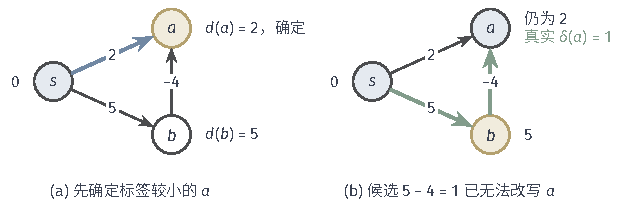
\includegraphics[width=105.583mm]{figures/01-basic-mathematics/04-graphs/tikz/c3-dijkstra-counterexample/figure.pdf}
  \caption{负边使Dijkstra算法过早确定标签。(a) 处理$s$后，$a$的标签$2$小于$b$的标签$5$，$a$被永久确定（黄色为当前出队顶点）。(b) 处理$b$时候选值$5-4=1$已无法改写$a$；真实最短路是$s\to b\to a$（绿色），成本$1$。图中没有负环，出错的原因是后半段弧$b\to a$为负。}
  \label{fig:graph-opt-dijkstra-counterexample}
\end{figure}

\paragraph{出队轨迹}
把四点图中$a\to b$的长度由$-1$改为$1$，全部弧长非负，Dijkstra算法适用。下面依次列出出队顶点与松弛结果：
\begin{enumerate}
  \item 取出$s$（标签$0$），松弛得$d(a)=2$、$d(b)=5$，前驱都是$s$；
  \item 取出$a$（标签$2$），候选$2+1=3<5$使$d(b)=3$、$p(b)=a$，候选$2+5=7$使$d(t)=7$、$p(t)=a$；
  \item 取出$b$（标签$3$），候选$3+2=5<7$使$d(t)=5$、$p(t)=b$；
  \item 取出$t$（标签$5$），没有出弧，队列为空。
\end{enumerate}
最终$\delta(a)=2$、$\delta(b)=3$、$\delta(t)=5$，从$t$沿前驱回溯得到$s\to a\to b\to t$。图~\ref{fig:graph-opt-dijkstra-trace}画出每次出队后的状态：已确定集合$R$逐个向外扩张，每个顶点在出队时的标签都不再改变。

\begin{figure*}[!htb]
  \centering
  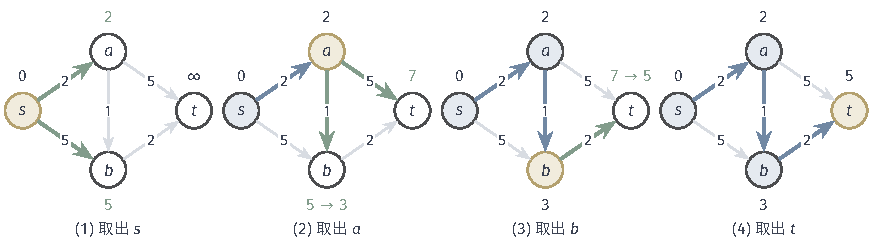
\includegraphics[width=147.687mm]{figures/01-basic-mathematics/04-graphs/tikz/c3-dijkstra-trace/figure.pdf}
  \caption{Dijkstra算法在非负四点图上的出队过程（$a\to b$长$1$，其余同前）。每个面板对应一次出队：蓝色为已确定顶点，黄色为本次出队的顶点，绿色标签与绿色弧表示本次松弛改善的标签及新前驱。四次出队依次确定$s=0$、$a=2$、$b=3$、$t=5$，最终前驱弧组成路线$s\to a\to b\to t$。}
  \label{fig:graph-opt-dijkstra-trace}
\end{figure*}

\paragraph{计算开销}
每个顶点至多出队一次，每条弧在其起点出队时松弛一次。用邻接表存储图、用支持降键的索引二叉堆存储未确定顶点时，取最小与降键各需$O(\log n)$时间，总时间为$O((n+a)\log n)$；标签、前驱、堆及其位置索引共占$O(n)$额外空间，图本身的存储另计。不降键的实现每次改善插入一个条目，堆中至多有$a+1$个条目，操作时间为$O(\log a)=O(\log n)$，总时间仍为$O((n+a)\log n)$，但队列空间上界变为$O(a)$。稠密图上也可以不用堆，每次扫描数组找最小标签，总时间为$O(n^2+a)$。

\subsection{方法比较与结果检验}
\label{sec:graph-opt-shortest-path-comparison}

三种算法解决同一个单源问题，但对输入的要求不同。比较它们时应先问：图有没有有向环？可达部分有没有负长度弧？是否需要检测负环？然后才比较运行时间。表~\ref{tab:graph-opt-shortest-path-methods}汇总了这些区别。

\begin{table}[!htb]
  \centering
  \caption{三种单源最短路算法的比较（$n$为顶点数，$a$为弧数，邻接表存储）。}
  \label{tab:graph-opt-shortest-path-methods}
  \begin{tabular}{llll}
    \toprule
    & 有向无环图递推 & Bellman--Ford & Dijkstra \\
    \midrule
    图结构 & 无有向环 & 不限 & 不限 \\
    弧长 & 任意实数 & 任意实数 & 可达部分非负 \\
    标签修正 & 处理后不变 & 反复修正 & 出队后不变 \\
    负环 & 不会出现 & 检测并标记 & 条件排除 \\
    时间 & $O(n+a)$ & $O(na)$ & $O((n+a)\log n)$ \\
    正确性依据 & 拓扑序归纳 & 至多$k$弧递推 & 首个未定顶点 \\
    \bottomrule
  \end{tabular}
\end{table}

“允许负边”与“存在负环”是两件不同的事。有向无环图递推与Bellman--Ford算法都允许负边；前者因为无环而不会遇到负环，后者则能在负环存在时正确报告受影响的顶点。Dijkstra算法连负边都不允许，哪怕负边并不构成负环，图~\ref{fig:graph-opt-dijkstra-counterexample}就是这样的例子。一种算法在某组数据上跑得更快、甚至答案碰巧正确，都不能替代对其条件的检查。

\paragraph{有限距离的检验}
拿到一份声称的最短路结果后，可以不重跑算法而直接核对。对标签有限的顶点，先沿前驱恢复路线，检查起点为$s$、终点为$v$、每一步都是原图中的弧，并重算弧长之和是否等于$d(v)$。这一步证明标签可以达到，即$d(v)\geq\delta(v)$。

最优性需要反方向的下界。若输出满足$d(s)=0$，并且对每条起点标签有限的弧$u\to v$都有
\[
  d(v)\leq d(u)+\ell_{u,v},
\]
那么任取一条$s$到$v$的行走$W=(s=w_0,w_1,\ldots,w_k=v)$，沿$W$把这些不等式逐条相加，中间标签相消，得到$d(v)\leq d(s)+\ell(W)=\ell(W)$。所以$d(v)\leq\delta(v)$，与可达性一起给出$d(v)=\delta(v)$。这组逐弧不等式只需$O(n+a)$时间核对，它本身就是有限距离的最优性证书；不满足时，违反不等式的弧直接指出了一条更好的路线。

\paragraph{不可达与负无穷的检验}
另外两类结果需要不同的证据。对报告为$+\infty$的顶点，用一次广度优先遍历核对它确实不在$s$的可达集中。对报告为$-\infty$的顶点，应给出三段证据：一条从$s$到某个有向环的行走、该环的成本为负，以及一条从环到该顶点的行走。三类结果各有各的验收方式，不能只核对其中一类就宣布整份结果正确。
